\documentclass[10pt]{article}
\usepackage{hyperref}
\hypersetup{
    colorlinks=true,
    linkcolor=black,
    filecolor=magenta,      
    urlcolor=cyan,
}

\usepackage{siunitx}
\usepackage{esvect}
\usepackage{fourier}
\usepackage{amssymb}
\usepackage{amsmath}
\usepackage{multicol}
\usepackage{geometry}
\usepackage[framemethod=TikZ]{mdframed}
\geometry{
 a4paper,
 total={160mm,237mm},
 left=30mm,
 top=30mm,
}

\usepackage{tikz}
\usetikzlibrary{automata, positioning, calc, through, angles, quotes, intersections}
\usepackage{multirow}

\author{Iker M. Canut}
\begin{document}
\title{Introducción a la Matemática}
\maketitle
\date
\newpage
\section{Conjuntos}
\subsection{Definiciones Básicas}
Un Conjunto es una colección de objetos. Los conjuntos se denominan con letras mayúsculas. Y los elementos que lo forman con letras minúsculas. El conjunto vacio se denomina $\emptyset$.
\subsection{Representación de conjuntos}
\begin{itemize}
\item \textbf{Por Extensión}: Se lista todo entre llaves. $\{a,b,c,d,...\}$
\item \textbf{Por Comprension}: Se dicen las propiedades. $\{x/x...\}$
\end{itemize}
\subsection{Subconjuntos}
El conjunto B es subconjunto de A si y sólo si todo elemento de B, es también de A.
\begin{center}
\framebox[8cm][c]{$B \subset A \iff (x \in B \Rightarrow x \in A) $}
\end{center}
Dos conjuntos serán iguales cuando posean los mismos elementos.
\begin{center}
\framebox[8cm][c]{$B = A \iff (A \subset B \land B \subset A) $}
\end{center}
Al conjunto que contiene a todos los datos en un contexto específico lo denominaremos \textbf{Conjunto\\ Universal} y se denota con la letra \textbf{U}.
\subsection{Operaciones}
\begin{itemize}
\item \textbf{Intersección de Conjuntos}: $A \cap B = \{x/x \in A \land x \in B\}$
\item \textbf{Unión de Conjuntos}: $A \cup B = \{x/x \in A \lor x \in B\}$
\end{itemize}
Si dos conjuntos no tienen elementos en comun, entonces son \textbf{disjuntos}. A y B disjuntos $\iff A \cap B = \emptyset$
\vspace{-.2cm}
\begin{table}[h]
\begin{center}
\begin{tabular}{|c|c|c|}
\hline
Propiedades&UNIÓN&INTERSECCIÓN\\
\hline
\textit{Conmutativa}&$A \cup B = B \cup A$&$A \cap B = B \cap A$\\
\hline
\textit{Asociativa}&$(A \cup B) \cup C = A \cup (B \cup C)$&$(A \cap B) \cap C = A \cap (B \cap C)$\\
\hline
\textit{Distributiva}&$A \cup (B \cap C) = (A \cup B) \cap (A \cup C)$&$A \cap (B \cup C) = (A \cap B) \cup (A \cap C)$\\
\hline
\textit{Idempotencia}&$A \cup A = A$&$A \cap A = A$\\
\hline
\end{tabular}
\end{center}
\end{table}
\vspace{-.2cm}
\begin{itemize}
\item \textbf{Diferencia}: $A - B = \{x/x \in A \land x \not \in B\}$
\item \textbf{Complemento}: $C_A = \overline{A} = U - A$. Se cumple que $A - B = A \cap \overline{B}$
\end{itemize}
\begin{table}[h]
\begin{center}
\begin{tabular}{|c|c|}
\hline
\multicolumn{2}{|c|}{Propiedades}\\
\hline
&\\
\multirow{4}{*}{\textit{Complemento}}&$\overline{\overline{A}} = A$\\&$A \cup \overline{A} = U$\\&$A \cap \overline{A} = \emptyset$\\&$\overline{\emptyset} = U \land \overline{U} = \emptyset$\\
&\\
\hline
&\\
\multirow{2}{*}{\textit{Leyes de Morgan}}&$\overline{A \cap B} = \overline{A} \cup \overline{B}$\\&$\overline{A \cup B} = \overline{A} \cap \overline{B}$\\
&\\
\hline
\end{tabular}
\end{center}
\end{table}
\begin{itemize}
\item \textbf{Cardinal de un conjunto}: Es el número de elementos. $|A| = card(A)$
\end{itemize}

\newpage
\section{Números Reales}
\begin{multicols}{2}
\begin{itemize}
\item \textbf{Naturales $N$}: $\{1,2,3,...\}$
\item \textbf{Naturales con cero $N_0$}: $\{0,1,2,3,...\}$
\item \textbf{Enteros $Z$}: $\{...,-3,-2,-1,0,1,2,3,...\}$
\item \textbf{Racionales $Q$}=$\left\{x/x=\frac{p}{q},p \in Z, q \in Z, q \not = 0\right\}$
\item \textbf{Irracionales $I$}=$Q \cap I = \emptyset \land Q \cup I = R$
\end{itemize}
\end{multicols}
\begin{quote}
\begin{center}
$N \subset N_0 \subset Z \subset Q \subset R \land I \subset R$
\end{center}
\end{quote}
\subsection{Potenciación}
\begin{multicols}{2}
\begin{itemize}
\item Si $a \not = 0, a^0 = 1$
\item $a^1 = a$
\item Si $n \in N, n>1, a^n = \underbrace{a.a. ... . a}_\text{n factores "a"}$
\item Si $a \in R \land a \not = 0 \land n \in N, a^{-n} = \dfrac{1}{a^n}=\dfrac{1}{\underbrace{a.a. ... . a}_\text{n veces}}$
\end{itemize}
\end{multicols}
\begin{table}[h]
\begin{center}
\begin{tabular}{|c|c|}
\hline
\textit{Distributiva respecto a la multiplicación}&$(a.b)^n=a^n.b^n$\\
\hline
\textit{Distributiva respecto al cociente}&$\left(\dfrac{a}{b}\right)^n = \dfrac{a^n}{b^n}, b \not = 0$\\
\hline
\textit{Producto de potencias de igual base}&$a^n.a^m = a^{n+m}$\\
\hline
\textit{Cociente de potencias de igual base}&$a^n \div a^m = a^{n-m}$\\
\hline
\textit{Potencia de potencia}&$\left(a^n\right)^m = a^{n.m}$\\
\hline
\end{tabular}
\end{center}
\end{table}
\subsection{Radicación}
$\sqrt[n]{a} = b \iff b^n=a$ \hfill y se nombra $\sqrt[indice]{radicando} =$ raiz enesima\\ \\
No existe en los reales la raiz cuadrada (y de ningún índice par) de números negativos. Es decir:
\begin{itemize}
\item Si \textbf{n} es un numero natural \textbf{impar}, entonces es valida para todo número real \textbf{a}.
\item Si \textbf{n} es un numero natural \textbf{par}, entonces es valida para todo número real \textbf{a no negativo}.
\end{itemize}
\begin{center}
\framebox[8cm][c]{$a^{\dfrac{m}{n}} = \sqrt[\scriptstyle{n}]{a^m} \land a^{-\dfrac{m}{n}} = \dfrac{1}{\sqrt[n]{a^m}}, a \not = 0$}
\end{center}
\begin{table}[h]
\begin{center}
\begin{tabular}{|c|c|}
\hline
\textit{Distributiva respecto al producto} & $\sqrt[n]{a.b} = \sqrt[n]{a}.\sqrt[n]{b}$\\
\hline
\textit{Distributiva respecto al cociente} & $\sqrt[n]{\dfrac{a}{b}} = \dfrac{\sqrt[n]{a}}{\sqrt[n]{b}}$\\
\hline
\textit{Raiz de raiz} & $\sqrt[m]{\sqrt[n]{a}} = \sqrt[m.n]{a}$\\
\hline
\end{tabular}
\end{center}
\end{table}
\newpage
\subsection{Logaritmo}
\textbf{El logaritmo en base a de x es y} y lo notamos $\log_a(x)=y$, como el numero al cual tengo que elevar a \textbf{a} para obtener \textbf{x}.
\begin{center}
$log_a(x)=y \iff a^y=x$, se necesita que $a>0 \land x>0 \land a \not = 1$
\end{center}
\begin{multicols}{2}
\begin{itemize}
\item $log_a(1)=0$
\item $log_a(a)=1$
\item $log_a(x.y)=log_a(x)+log_a(y)$
\item $log_a{\left(\dfrac{x}{y}\right)}=log_a(x)-log_a(y)$
\item $log_a(x^c) = c.log_a(x)$
\item $a^{log_a(x)}=x$
\end{itemize}
\end{multicols}
\begin{center}
\framebox[8cm][c]{$log_b(x) = \dfrac{log_a(x)}{log_a(b)}$}
\end{center}
\subsection{Formas Especiales}
\textbf{Binomio al Cuadrado $\leftrightarrow$ Trinomio Cuadrado Perfecto}
\begin{center}
\framebox[8cm][c]{$(x+y)^2 = x^2+2xy+y^2$}
\end{center}
\textbf{Binomio al Cubo $\leftrightarrow$ Cuatrinomio Cubo Perfecto}
\begin{center}
\framebox[8cm][c]{$(x+y)^3 = x^3+3x^2y+3xy^2+y^3$}
\end{center}
\textbf{Diferencia de Cuadrados}
\begin{center}
\framebox[8cm][c]{$(a-b).(a+b)=a^2-b^2$}
\end{center}
\subsection{Relacion de Orden del Conjunto de los Numeros Reales}
\begin{multicols}{3}
\begin{itemize}
\item $a<b$ si $0<b-a$
\item $a>b$ si $b<a$
\item $a<b \land b<c \Rightarrow a<c$
\item $a<b \Rightarrow a+c<b+c$
\item $a<b \land c>0 \Rightarrow a.c<b.c$
\item $a<b \land c<0 \Rightarrow a.c>b.c$
\end{itemize}
\end{multicols}
\subsection{Valor Absoluto}
Es la distancia que hay, en la recta numérica, desde su punto representativo al origen de coordenadas. El valor absoluto es será siempre un número positivo (o cero).
\[|x| = \left\{ \begin{array}{ll}
x  &$ si $x \geq 0\\
-x &$ si $x < 0\\
\end{array}\right.\]\
\begin{multicols}{2}
\begin{itemize}
\item $|a| \geq 0$
\item $|a|.|b| = |a|.|b|$
\item $|a|=0 \iff a=0$
\item $\left|\dfrac{a}{b}\right| = \dfrac{|a|}{|b|}, b \not = 0$
\item $|-a| = |a|$
\item $\sqrt{a^2} = |a|$
\end{itemize}
\end{multicols}
$\forall a, b \in R \land k>0$
\begin{multicols}{2}
\begin{itemize}
\item $|a+b| \leq |a| + |b|$
\item $|a-b| \geq ||a|-|b||$
\item $|a|<k \iff -k < a < k$
\item $|a|>k \iff (a>k \lor a<(-k))$
\end{itemize}
\end{multicols}

\newpage
\section{Números Complejos}
Se define $i$ como: \hspace{4cm} \framebox[2cm][c]{$i^2 = -1$}
\subsection{Forma Binómica de un Número Complejo}
\begin{center}
\framebox[2cm][l]{$z = a+bi$}\hfill donde \textbf{a} y \textbf{b} son numeros reales, e \textbf{i} se define por la relacion $i^2=-1$
\end{center}
El numero \textbf{a} = $Re(z)$ es la parte real de z y \textbf{b} = $Im(z)$ es la parte imaginaria de z.
\subsection{La Unidad Imaginaria}
El número \textbf{i} recibe el nombre de unidad imaginaria, aceptandose que se comporta como un número real.
\begin{multicols}{3}
\begin{itemize}
\item $i^r.i^s = i^{r+s}$
\item $(i^r)^s = i^{r.s}$, con $r,s \in Z$
\item $i^0 = 1$
\item $i^1 = i$
\item $i^2 = -1$
\item $i^3 = -i$
\end{itemize}
\end{multicols}
\begin{center}
\framebox[8cm][c]{$i^n = i^r$, donde r=n\%4}
\end{center}
\subsection{El conjunto de los Números Complejos}
Se simboliza con la C y contiene los números de la forma $a+bi$, donde $a,b \in R$ e \textbf{i} es la unidad imaginaria.
\begin{center}
\framebox[8cm][c]{$C = \{z=a+bi/a,b \in R \land i^2 = -1\}$}
\end{center}
\begin{itemize}
\item Los números reales son complejos $R \subset C$, ya que si $x \in R \Rightarrow x = x+0i$.
\item A los complejos de la forma $bi$ (aquellos que su parte real es nula), se los llama imaginarios puros.
\end{itemize}
\subsection{Definiciones}
\begin{itemize}
\item \textbf{Igualdad de Números Complejos}: $z_1=z_2 \iff (a_1=a_2 \land b_1=b_2)$.
\item \textbf{Opuesto de un Número Complejo}: $-z=(-a)+(-b)i$.
\item \textbf{Suma y Resta}: $z_1+z_2 = (a_1+a_2)+(b_1+b_2)i$. De manera analoga, $z_1-z_2 = (a_1-a_2)+(b_1-b_2)i$
\item \textbf{Multiplicación}: $z_1.z_2 = (a_1.a_2-b_1.b_2) + (a_2.b_1+a_1.b_2)i$.
\item \textbf{División}: $\dfrac{a+bi}{c+di} = \dfrac{ac+bd}{c^2+d^2}+\dfrac{bc-ad}{c^2+d^2}i$
\end{itemize}
\subsection{Conjugado de un complejo}
El conjugado de un número complejo $z=a+bi$ es $\overline{z}=a-bi$.
\begin{itemize}
\begin{multicols}{3}
\item $z = \overline{z} \iff z \in R$
\item $z + \overline{z} = 2a$
\item $z - \overline{z} = 2bi$
\item $\overline{z_1 + z_2} = \overline{z_1} + \overline{z_2}$
\item $\overline{z_1 . z_2} = \overline{z_1} . \overline{z_2}$
\item $- \overline{z} = \overline{-z}$
\item $z . \overline{z} = a^2 + b^2 = Re(z)^2 + Im(z)^2$
\end{multicols}
\end{itemize}
\subsection{Reciproco de un Complejo NO nulo}
Definimos el reciproco de $z \not = 0, z \in C$, como aquel complejo $w$ / $z \times w=1$ y lo denotamos $z^{-1} = \frac{1}{z}$.
\begin{multicols}{2}
\begin{itemize}
\item $\overline{\left(\dfrac{z_1}{z_2}\right)} = \dfrac{\overline{z_1}}{\overline{z_2}}, z_2 \not = 0$
\item $\overline{\left(\dfrac{1}{z}\right)} = \dfrac{1}{\overline{z}}, z \not = 0$
\end{itemize}
\end{multicols}

\newpage
\section{Ecuaciones e Inecuaciones}
Una \textbf{ecuación} es una igualdad entre dos expresiones algebraicas: $P(x)=Q(x)$. Resolverla consta de encontrar el o los valores numéricos de la incógnita que verifican la ecuación.
\subsection{Ecuaciones Lineales}
Una ecuación es \textbf{lineal} cuando se puede escribir de la forma: \hfill \framebox[5cm][c]{$a.x+b=0$, con $a \not = 0$}
\subsection{Ecuaciones Cuadráticas}
Una ecuación es \textbf{cuadratica} cuando se puede escribir de la forma: \hfill \framebox[5cm][c]{$a.x^2+b.x+c=0$, con $a \not = 0$}\\
\begin{center}
\framebox[8cm][c]{$x_{1,2} = \dfrac{-b \pm \sqrt{b^2 - 4ac}}{2a}$}
\end{center}
El numero $\vartriangle = b^2-4ac$ se llama \textbf{\textit{discriminante}} y decide la naturaleza de las soluciones.
\begin{itemize}
\item Si $\vartriangle > 0$ entonces las dos soluciones son reales y distintas.\\
\item Si $\vartriangle = 0$ entonces tiene una solución doble.\\
\item Si $\vartriangle < 0$ entonces las dos soluciones son numeros complejos conjugados.
\end{itemize}
\begin{table}[h]
\begin{center}
\begin{tabular}{|c|}
\hline
\\
$x_1+x_2 = -\dfrac{b}{a}$\\
\\
$x_1.x_2 = \dfrac{c}{a}$\\
\\
\hline
\end{tabular}
\end{center}
\end{table}
\subsection{Ecuaciones Bicuadrática}
Una ecuación es \textbf{bicuadratica} cuando se puede escribir de la forma: \hfill \framebox[5cm][c]{$a.x^4+b.x^2+c=0$, con $a \not = 0$}\\
Para resolverlas, primero se sustituye $y=x^2$ y despues se sigue normal.
\subsection{Inecuaciones}
Una \textbf{inecuación} es una desigualdad entre dos expresiones algebraicas: $P(x) \leq Q(x)$. Resolverla consta de encontrar el o los valores numéricos de la incógnita que verifican la ecuación.

\newpage
\section{Geometría}
\subsection{Ángulos Determinados por Dos Rectas y Una Transversal}
\begin{multicols}{2}
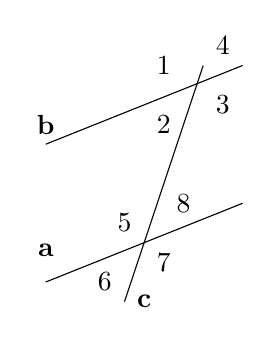
\begin{tikzpicture}[scale=.5]
\draw (0,5) -- (5,7);
\draw (0,1.5) -- (5,3.5);
\draw (2,1) -- (4,7);
\node at (3,7){$\widearc{1}$};
\node at (3,5.5){$\widearc{2}$};
\node at (4.5,6){$\widearc{3}$};
\node at (4.5,7.5){$\widearc{4}$};
\node at (2,3){$\widearc{5}$};
\node at (1.5,1.5){$\widearc{6}$};
\node at (3,2){$\widearc{7}$};
\node at (3.5,3.5){$\widearc{8}$};
\node at (0,2.3){\textbf{a}};
\node at (0,5.5){\textbf{b}};
\node at (2.5,1){\textbf{c}};
\end{tikzpicture}
\begin{itemize}
\item $\widearc{2}$ y $\widearc{8}$ son alternos internos
\item $\widearc{4}$ y $\widearc{6}$ son alternos externos
\item $\widearc{4}$ y $\widearc{8}$ son correspondientes
\item $\widearc{3}$ y $\widearc{8}$ son conjugados internos
\item $\widearc{4}$ y $\widearc{7}$ son conjugados externos
\item $\widearc{1}$ y $\widearc{3}$ son opuestos por el vértice
\end{itemize}
\end{multicols}
\begin{itemize}
\item Los ángulos correspondientes son congruentes $\iff$ las rectas a y b son paralelas.
\item Los ángulos opuestos por el vértice son congruentes.
\item Los ángulos alternos internos (externos) son congruentes $\iff$ las rectas a y b son paralelas.
\item Los ángulos conjugados internos (externos) son suplementarios $\iff$ las rectas a y b son paralelas.
\end{itemize}
\subsection{Triángulos}
- Los triángulos se pueden clasificar...
\begin{multicols}{2}
\begin{itemize}
\item \textbf{según sus lados:}
\begin{itemize}
\item Equilátero
\item Isósceles
\item Escaleno
\end{itemize}
\item \textbf{según sus ángulos:}
\begin{itemize}
\item Acutángulo
\item Rectángulo
\item Obtusángulo
\end{itemize}
\end{itemize}
\end{multicols}
\vspace{.5cm}
- Los elementos de un triángulo son:
\begin{itemize}
\item \textbf{Mediana}: es el segmento que une el punto medio de un lado con el vértice opuesto al mismo.
\item \textbf{Mediatriz}: es una recta perpendicular a un lado que pasa por su punto medio.
\item \textbf{Altura}: es el segmento perpendicular a un lado que pasa por su vértice opuesto.
\item \textbf{Bisectriz}: es la bisectriz de un ángulo.
\end{itemize}
\vspace{1cm}
- Y algunos puntos notables de un triángulo son:
\begin{itemize}
\item \textbf{Baricentro}: Las medianas se intersecan en un punto llamado baricentro, tal que su distancia a cada vértice es el doble a la distancia al punto medio del lado opuesto.
\item \textbf{Circuncentro}: Las mediatrices se intersecan en un punto llamado circuncentro, que es el centro de la circunferencia circunscripta al triángulo.
\item \textbf{Ortocentro}: Las rectas que contienen a las alturas se intersecan en un punto denominado ortocentro.
\item \textbf{Incentro}: Las bisectrices se intersecan en un punto denominado incentro, que es el centro de una circunferencia inscripta en el triángulo.
\end{itemize}
\subsection{Algunas Propiedades Importantes}
\begin{itemize}
\item En un $\triangle$ cada lado es menor que la suma de los otros dos, y mayor que su diferencia.
\item La suma de los ángulos interiores de un $\triangle$ es igual a un llano (180º).
\item El ángulo exterior a un $\triangle$ es igual a la suma de los dos interiores no adyacentes a él.
\item En un $\triangle$, a lados congruentes se oponen ángulos congruentes y viceversa.
\item En un $\triangle$, a mayor lado se opone mayor ángulo y viceversa.
\end{itemize}
\subsection{Congruencia de Triángulos}
Dos triángulos son \textbf{\textit{congruentes}} si tienen su lados y su ángulos respectivamente congruentes.\\ Dos triángulos son congruentes $\iff$
\begin{itemize}
\item Sus \textbf{tres lados} son respectivamente congruentes.
\item \textbf{Dos de sus lados y el ángulo comprendido} entre ellos son respectivamente congruentes. 
\item \textbf{Un lado y los ángulos con vértice en los extremos de dicho lado} son respectivamente congruentes.
\item \textbf{Dos de sus lados y el ángulo opuesto al mayor de los lados} son respectivamente congruentes.
\end{itemize}
\subsection{Semejanza de Triángulos}
Dos $\triangle$ son \textbf{\textit{semejantes}} si tienen sus ángulos congruentes y sus lados homólogos proporcionales.\\
Dos triángulos son semejantes $\iff$
\begin{itemize}
\item Sus \textbf{tres lados} son proporcionales.
\item \textbf{Dos de sus lados} son proporcionales \textbf{y los ángulos comprendidos} entre ellos son congruentes.
\item \textbf{Tiene un par de ángulos} respectivamente congruentes.
\end{itemize}
\subsection{Polígonos (de más de tres lados)}
\textbf{Propiedades de polígonos convexos}:\\
La suma de los ángulos interiores de un polígono de $n$ lados se representa como:
\begin{center}
\framebox[8cm][c]{$S_n = (n-2) . 180$º}
\end{center}
Esto es porque la suma de los ángulos exteriores de un polígono de n lados es igual a 360º.
\subsection{Circunferencias}
Se define a una circunferencia como el lugar geométrico de los puntos del plano que equidistan de uno fijo, llamado centro. Las posiciones relativas de una recta y una circunferencia, y entre dos circunferencias, son:
\begin{itemize}
\item Una recta es \textbf{exterior} a una circunferencia si no tienen puntos en común.
\item Una recta es \textbf{tangente} a una circunferencia si tienen \textbf{solo} un punto en común.
\item Una recta es \textbf{secante} a una circunferencia si se intersecan en dos puntos.
\item Dos circunferencias son \textbf{secantes} si tienen dos puntos en común.
\item Dos circunferencias son \textbf{tangentes} si tienen solo un punto en común.
\item Dos circunferencias son \textbf{conceéntricas} si tienen el mismo centro.
\end{itemize}
\newpage
\subsection{Elementos de una Circunferencia}
\begin{multicols}{2}
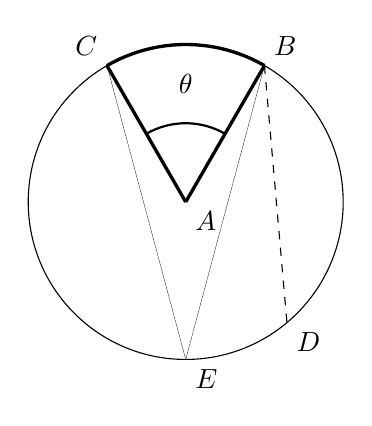
\begin{tikzpicture}[scale=2]
\coordinate [label=below right: $A$] (A) at (0,0);
\node[draw] (ci) at (A) [circle through=(right:1)] {};
\coordinate [label=above left:$C$] (C) at (ci.120);
\draw [very thick] (C) -- (A);
\coordinate [label=above right:$B$] (B) at (ci.60);
\draw [very thick] (B) -- (A);
\coordinate [label=below right:$ D$] (D) at (ci.310);
\draw [dashed] (B) -- (D);
\draw [black, very thick, domain=120:60] plot ({cos(\x)}, {sin(\x)});

\coordinate [label=below right:$E$] (E) at (ci.270);
\draw [ultra thin] (B)--(E);
\draw [ultra thin] (C)--(E);
\pic ["$\theta$", draw=black, thick, -, angle eccentricity=1.5, angle radius=1cm] {angle = B--A--C};
\end{tikzpicture}
\begin{itemize}
\item \textbf{BD Cuerda}, segmento cuyos extremos están en la circunferencia.
\item \textbf{CD Diámetro}, mayor de las cuerdas y contiene al centro de la circunferencia.
\item \textbf{AC Radio}, segmento cuyos extremos son el centro de la circunferencia y un punto de la misma.
\item \textbf{$\widearc{CB}$ arco}, subconjunto de la circunferencia.
\end{itemize}
\end{multicols}
\begin{itemize}
\item \textbf{$C\hat{A}B$ ángulo central} que se relaciona con el arco $\widearc{CB}$ es un ángulo cuyo vértice es el centro de la circunferencia y sus lados pasan por los extremos del arco al cual se lo relaciona.
\item \textbf{$C\hat{E}B$ ángulo inscripto} en la circunferencia que abarca el arco $\widearc{CB}$, es un ángulo cuyo vértice está en la circunferencia y sus lados pasan por los extremos del arco al cual se lo relaciona.
\end{itemize}
Propiedades:
\begin{itemize}
\item \framebox[2.5cm][c]{$C\hat{E}B = \dfrac{1}{2}C\hat{A}B$} Un ángulo inscripto es congruente con la mitad del central que abarca el mismo arco.
\item \framebox[2.5cm][c]{$C\hat{E}B = C\hat{D}B$} Los ángulos inscriptos en un mismo arco son congruentes.\\
\end{itemize}
\subsection{Perímetros}
\begin{itemize}
\item El \textbf{perímetro} de un polígono de $n$ lados es la suma de las longitudes de cada uno de los $n$ lados
\item La \textbf{longitud} de una circunferencia de radio $R$ es $2 \pi R$.
\end{itemize}
\subsection{Áreas}
\begin{itemize}
\item Un triangulo de base $b$ y altura $h$ es igual a: $\dfrac{b \times h}{2}$
\item Un paralelogramo de base $b$ y altura $h$ es igual a: $b \times h$.
\item Un trapecio de base mayor $B$ y de base menor $b$ y altura $h$ es: $\dfrac{(B + b) \times h} {2}$.
\item Un rombo cuyas diagonales miden $D$ y $d$ es: $\dfrac{D \times d}{2}$.
\item Un polígono regular de $n$ lados que miden $l$ y apotema $ap$ es: $\dfrac{n \times l \times ap}{2}$
\item Una circunferencia de radio $R$ es: $\pi R^2$.
\end{itemize}
\newpage
\subsection{Cuerpos}
Los poliedros son cuerpos cuyas caras son polígonos.\\
\textbf{Teorema de Euler}: Establece que en un poliedro convexo el número de caras, más los vértices menos las aristas es siempre igual a 2: $f+v-e = 2$\\
\textbf{Algunos poliedros particulares}:
\begin{itemize}
\item \textbf{Prisma}: Es un poliedro que tiene dos caras que son poligonos congruentes, contenidas en planos paralelos. Los prismas rectos son aquellos cuyas caras laterales son rectangulos. La altura de un prisma es la distancia entre las bases. Un \textbf{paralelepipedo} es un prisma de seis caras, cuyas bases son paralelogramos, iguales y paralelos dos a dos. Un paralelepipedo en el que todas sus bases son rectangulos y por tanto todas sus caras son perpendiculares entre si, es un \textbf{paralelepipedo recto}.
\item \textbf{Piramide}: es unn poliedro que tiene una cara (llamada base) que es un poligono cualquiera y las otras caras concurren en un punto (llamado vertice), en efecto, son triangulos. Hay tantas caras laterales como lados tenga la base. Las \textbf{Piramides rectas} son aquellas cuyas caras laterales son triangulos isosceles y el pie de la altura esta en el centro de la base.
\end{itemize}
\textbf{Poliedros regulares}
Son poliedros regulares aquellos cuyas caras son poligonos regulares congruentes, y a cada vértice concurren el mismo numero de aristas. Solo hay 5 poliedros regulares:
\begin{table}[h]
\begin{center}
\begin{tabular}{|c|c|c|}
\hline
Poliedro Regular & Nº de Caras & Forma caras \\
\hline
Tetraedro & 4 & Triangulo equilatero\\
Cubo & 6 & Cuadrado\\
Octaedro & 8 & Triangulo equilatero\\
Dodecaedro & 12 & Pentagono regular\\
Icosaedro & 20 & Triangulo equilatero\\
\hline
\end{tabular}
\end{center}
\end{table}
\subsection{Cuerpos Redondos}
Son cuerpos redondos la esfera, el cilindro (oblicuo, recto) y el cono (oblicuo, -).\\
\subsection{Volumenes de cuerpos}
\begin{itemize}
\item Prismas y cilindros: $area\ de\ la\ base \times altura$
\item Piramides y conos: $\dfrac{area\ de\ la\ base \times altura}{3}$
\item Esfera: $\dfrac{4}{3} \times \pi \times r^{3}$
\end{itemize}
\subsection{Áreas de Cuerpos}
Si los cuerpos son poliedros, hallar el area de los mismos es sumar las areas de cada una de sus caras. En el caso de prismas y piramides el area total se divide en area lateral y area de las bases.\\ \\
El area de una esfera de radio R se obtiene mediante: $4 \times \pi \times R^2$.\\ \\
El area de un cilindro recto de base de radio R y altura h con sus dos bases se obtiene mediante:
\begin{center}
$2\ area_{base} + area_{lateral} = 2\ \times \pi \times R^2 + 2 \times \pi \times R \times h$
\end{center}

\newpage
\section{Trigonometría}
\subsection{Triangulos rectángulos: Razones Trigonométricas de ángulos agudos}
\begin{multicols}{3}
$sen(\hat{A}) = \dfrac{cateto\ opuesto\ a \ \hat{A}}{hipotenusa}$\\
$cos(\hat{A}) = \dfrac{cateto\ adyacente\ a \ \hat{A}}{hipotenusa}$\\
$tg(\hat{A}) = \dfrac{cateto\ opuesto\ a \ \hat{A}}{cateto\ adyacente\ a \ \hat{A}}$
\end{multicols}
\subsection{Resolución de triángulos cualesquiera}
\begin{table}[h]
\begin{center}
\begin{tabular}{cc}
Teorema del seno:& $\dfrac{a}{sen(\hat{A})} = \dfrac{b}{sen(\hat{B})} = \dfrac{c}{sen(\hat{C})}$\\ \\
Teorema del coseno & $a^2 = b^2 + c^2 - 2bc.cos(\hat{A})$
\end{tabular}
\end{center}
\end{table}
\subsection{Funciones Trigonométricas}
\begin{multicols}{2}
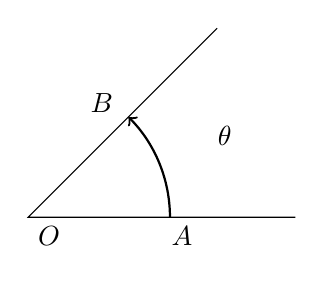
\begin{tikzpicture}[scale=.6]
\coordinate [label=below right: $O$] (O) at (0,0);
\coordinate [label=above left: $B$] (B) at (2,2);
\coordinate [label=below right: $A$] (A) at (2.828,0);
\coordinate (C) at (4,4);
\coordinate (D) at (5.656,0);

\draw (C)--(O)--(D);

\pic ["$\theta$", draw=black, thick, ->, angle eccentricity=1.5, angle radius=1.8cm] {angle = A--O--B};
\end{tikzpicture}\\
Consideremos la semirrecta $\vv{OA}$ girando alrededor de O hasta llegar a la posicion $\vv{OB}$. Decimos que esta rotacion ha generado el angulo $A\hat{O}B$, de vertice O y lado inicial $\vv{OA}$ y lado final$\vv{OB}$.\\ \\ El ángulo es positivo si ha sido generado en sentido contrario a las agujas del reloj.
\end{multicols}
Si el arco $\widearc{AB}$ generado por la rotacion del punto A es una circunferencia, diremos que el angulo generado es de una vuelta.\\
\begin{table}[h]
\begin{center}
\begin{tabular}{|c|}
\hline \\
Dos angulos $\alpha$ y $\beta$ son \textbf{congruentes} y se simboliza $\alpha \equiv \beta$ si tienen el mismo lado inicial y final\\ \\
\hline
\end{tabular}
\end{center}
\end{table}

Observaciones:
\begin{itemize}
\item El ángulo nulo y pleno son congruentes.
\item Para que ocurra la coincidencia de lados iniciales y finales, los ángulos congruentes deben diferir en una cantidad entera de vueltas. (Entera, no natural, porque puede ser negativa).
\end{itemize}

\subsection{Sistemas de Medición de Ángulos}
\subsubsection{Sistema Sexagesimal}
La unidad es el grado. Un ángulo de un grado equivale a $\frac{1}{360}$ del angulo de una vuelta.
\subsubsection{Sistema Radial}
La unidad es el radian y se define como la medida de un angulo central de una circunferencia.
\subsubsection{Relaciones}
Si llamamos x a la medida en radianes de un angulo que subtiende un arco $\widearc{AB}$ y llamamos $L$ a la longitud del mismo, tenemos que: $L = x.R$, es decir, $x=\dfrac{L}{R}$. Consecuentemente, si llamamos $\alpha$ a un angulo de una vuelta, la longitud del arco que subtiende coincide con la longitud de la circunferencia de radio R, por lo que: $\alpha = \dfrac{2 \pi R}{R} = 2 \pi$. De modo que \framebox[3cm][c]{$2 \pi rad \leftrightarrow \ang{360}$}
\newpage
\subsection{Funciones trigonométricas}
Las deficiones de las razones trigonometricas las podemos hacer extensivas a angulos no agudos y orientados por medio de la llamada "Circunferencia Trigonometrica" (Radio 1 y centro en el origen de coordenadas).
\begin{multicols}{2}
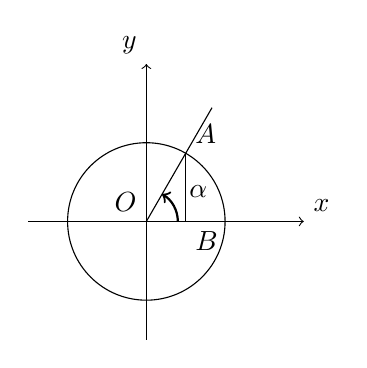
\begin{tikzpicture}[scale=1, one end extended/.style={shorten >=-1#1}, one end extended/.default=9]
\coordinate [label=above left: $y$] (Y) at (0,2);
\coordinate (YY) at (0,-1.5);
\draw [->] (YY) -- (Y);
\coordinate [label=above right: $x$] (X) at (2,0);
\coordinate (XX) at (-1.5,0);
\draw [->] (XX) -- (X);

\coordinate [label=above left: $O$] (O) at (0,0);
\node [draw] (ci) at (O) [circle through=(right:1)] {};
\coordinate [label=above right:$A$] (A) at (ci.60);

\coordinate [label=below right:$B$] (B) at (A|-O);

\draw (A) -- (B);
\draw [one end extended] (O) -- (A);
\pic ["$\alpha$", draw=black, thick, ->, angle eccentricity=1.9, angle radius=.4cm] {angle = B--O--A};
\end{tikzpicture}

Si tomamos un angulo $\alpha$, cuyo lado final interseca a la circunferencia trigonometrica en un punto A con coordenadas positivas (a,b), el punto B de coordenadas (a;0), tendremos el triangulo \(\overset{\triangle}{AOB}\) que es rectánguo en B. Por lo que tendremos que se cumplen las siguientes razones trigonométricas:
\end{multicols}
\begin{multicols}{3}
$sen(\alpha) = \dfrac{AB}{OA} = \dfrac{b}{1} = b$\\
$cos(\alpha) = \dfrac{OB}{OA} = \dfrac{a}{1} = a$\\
$tg(\alpha) = \dfrac{AB}{OB} = \dfrac{b}{a}$
\end{multicols}
Generalizando a cualquier angulo $\alpha$, diremos que $a=cos(\alpha)\ y\ b=sen(\alpha)$
\begin{table}[h]
\begin{center}
\begin{tabular}{|c|c|c|c|c|}
\hline
$\alpha$&$I_c$&$II_c$&$III_c$&$IV_c$\\
\hline
Coordenadas&$x>0 \land y>0$&$x<0 \land y>0$&$x<0 \land <0$&$x>0 \land y<0$\\
\hline
$sen\ \alpha$&+&+&-&-\\
\hline
$cos\ \alpha$&+&-&-&+\\
\hline
\end{tabular}
\end{center}
\end{table}

El valor del seno y el coseno es independiente de la circunferencia que se tome.
\subsubsection{Propiedades del seno y el coseno}
\begin{itemize}
\item \textbf{Acotación del seno y el coseno}: $-1 \leq sen(\alpha) \leq 1 \land -1 \leq cos(\alpha) \leq 1$
\item \textbf{Periodicidad del seno y el coseno}: $sen(\alpha + 2\pi) = sen(\alpha) \land cos(\alpha + 2\pi) = cos(\alpha)$
\item \textbf{Paridad del coseno e imparidad del seno}: $cos(-\alpha) = cos(\alpha) \land sen(-\alpha) = -sen(\alpha)$
\item \textbf{Relacion Pitagorica}: $sen^2(\alpha)+cos^2(\alpha) = 1$
\item \textbf{Relacion entre el seno y coseno de complementarios}: $sen \left(\dfrac{\pi}{2} - \alpha \right) = cos(\alpha) \land cos\left(\dfrac{\pi}{2}-\alpha \right) = sen(\alpha)$
\end{itemize}
\subsection{Funciones Reciprocas}
\begin{itemize}
\item $cotangente\ de\ x = ctg\ x = \dfrac{cos\ x}{sen\ x}$
\item $secante\ de\ x = sec\ x = \dfrac{1}{cos\ x}$
\item $cosecante\ de\ x = cos\ x = \dfrac{1}{sen\ x}$
\end{itemize}

\subsection{Razones Trigonométricas de suma o diferencia de ángulos}
\begin{itemize}
\item $cos\left(\alpha + \beta \right) = cos(\alpha).cos(\beta)-sen(\alpha).sen(\beta)$
\item $cos\left(\alpha - \beta \right) = cos(\alpha).cos(\beta)+sen(\alpha).sen(\beta)$
\item $sen\left(\alpha + \beta \right) = sen(\alpha).cos(\beta)+cos(\alpha).sen(\beta)$
\item $sen\left(\alpha - \beta \right) = sen(\alpha).cos(\beta)-cos(\alpha).sen(\beta)$
\item $cos(2\alpha) = cos^2(\alpha)-sen^2(\alpha)$
\item $sen(2\alpha) = 2sen(\alpha).cos(\alpha)$
\end{itemize}

\section{Sistemas de Ecuaciones}
\subsection{Sistemas de Ecuaciones Lineales}
\framebox[15cm][c]{Un sistema de ecuaciones es lineal cuando las ecuaciones que lo conforman son lineales}
\[(S) = \left\{ \begin{array}{ll}
a_{11} x_1 + a_{12} x_2 + a_{13} x_3 + ... + a_{1n} x_n = b1\\
a_{21} x_1 + a_{22} x_2 + a_{23} x_3 + ... + a_{2n} x_n = b2\\
...\\
a_{m1} x_1 + a_{m2} x_2 + a_{m3} x_3 + ... + a_{mn} x_n = bm\\
\end{array}\right.\]\
(S) es un sistema de $m$ ecuaciones lineales, con $n$ incognitas $x1;x2;x3;...;xn$, donde los coeficientes\\ $a_{i,j} \in R \forall i=1;2;...;m$ y $j=1;2;...;n$. Se dice que (S) es un sitema $m \times n$
\subsubsection{Posiciones Relativas entre dos rectas en el plano}
\begin{center}
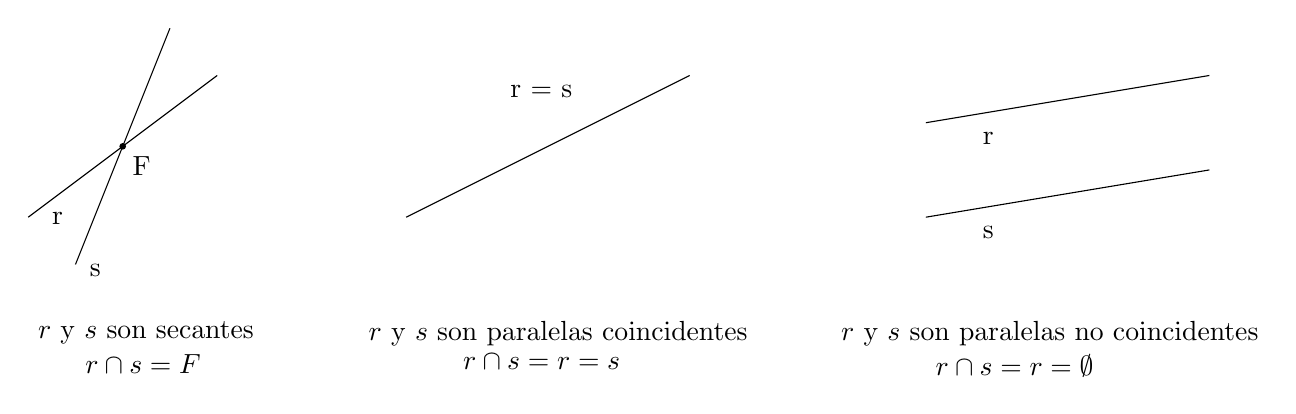
\begin{tikzpicture} [scale=0.6, every node/.style={black, below right}]
\draw [name path= line 1](0,1) -- (4,4);
\draw [name path= line 2](1,0) -- (3,5);
\fill[black, name intersections={of=line 1 and line 2, total=\t}]
	%\foreach \s in {1,...,\t}{(intersection-\s) circle (2pt) node {\s}};
	\foreach \s in {1,...,\t}{(intersection-\s) circle (2pt) node {F}};
\node at (0.3,1.3){r};
\node at (1.1,0.2){s};
\node at (0,-1){$r$ y $s$ son secantes};
\node at (1,-1.7){$r \cap s = {F}$};

\draw (8,1) -- (14,4);
\node at (10,4){r = s};
\node at (7,-1){$r$ y $s$ son paralelas coincidentes};
\node at (9,-1.7){$r \cap s = r = s$};

\draw (19, 1) -- (25, 2);
\draw (19, 3) -- (25, 4);
\node at (20,1){s};
\node at (20,3){r};
\node at (17,-1){$r$ y $s$ son paralelas no coincidentes};
\node at (19,-1.7){$r \cap s = r = \emptyset$};
\end{tikzpicture}
\end{center}
\vspace{.5cm}
A partir de esto podemos clasificar cada uno de los sistemas según la cantidad de soluciones:
\begin{itemize}
\item Cuando un sistema tiene solución diremos que es \textbf{COMPATIBLE}.
\begin{itemize}
\item Cuando la solución es unica, será \textbf{DETERMINADO}.
\item Cuando las soluciones son infinitas, será \textbf{INDETERMINADO}.
\end{itemize}
\item Cuando el sistema no tenga solución diremos que es \textbf{INCOMPATIBLE}.
\end{itemize}
\subsection{Para demostrar analiticamente las soluciones}
\subsubsection{Método por Sustitución}
Consiste en despejar una de las incognitas en función de la otra en una ecuacion y usar esa igualdad en la otra ecuación, sustituyendo la incógnita.
\subsubsection{Método por Igualación}
Consiste en despejar la misma incógnita en funcion de la otra en ambas ecuaciones, y finalmente, por propiedad transitiva, igualar.
\subsection{Definiciones}
\begin{itemize}
\item Cuando los términos independientes son todos nulos, decimos que el sistema es \textbf{homogéneo}. Es siempre compatible por tener al menos como solución la trivial (0;0;...;0).
\item Dos sistemas son \textbf{equivalentes} cuando tienen el mismo conjunto solución.
\item Un sistema es \textbf{escalonado} si cada eqn empieza con al menos un coeficiente nulo mas que la anterior.
\end{itemize}
\subsection{¿Cómo sabemos que sustituimos un sistema por otro equivalente?}
\begin{itemize}
\item Intercambiar ecuaciones
\item Multiplicar las ecuaciones del sistema por un número real no nulo
\item Sumar ecuaciones
\end{itemize}
\subsubsection{Método de Eliminación Gaussiana}
Se escalona y se resuelve el sistema usando operaciones elementales:
\begin{enumerate}
\item $(E_1) \times m - (E_2) \mapsto (E_2)$
\item $(E_1) \times n - (E_3) \mapsto (E_3)$
\item $(E_2) \times o - (E_3) \times p \mapsto (E_3)$
\end{enumerate}
\subsubsection{Algoritmo de Gauss}
\begin{table}[h]
\begin{multicols}{2}
\begin{tabular}{ccc|cc}
x&y&z& t.i.&\\
\hline
$\textbf{1}$&$\textbf{2}$&$-1$&$-5$&$E_1$\\
$\textbf{2}$&$\textbf{-1}$&$2$&$8$&$E_2$\\
$3$&$3$&$4$&$5$&$E_3$\\
\hline
&$\textbf{-5}$&$4$&$18$&$E_2'$\\
&$-3$&$7$&$20$&$E_3'$\\
\hline
&&$-23$&$-46$&$E_3''$\\
\end{tabular}

Para calcular los números se resuelven los determinantes 2x2 y se anota el resultado debajo, cancelando un término y escalonando el sistema:\\
$\begin{vmatrix}
1&2\\
2&-1
\end{vmatrix} = 1 \times (-1) - 2 \times 2 = \textbf{-5}$
\end{multicols}
\end{table}
\begin{itemize}
\item Si al final queda $0\ |\ 0$, implica que es \textbf{compatible determinado}.
\item Si al final queda $0\ |\ X\ \forall X \not = 0$, implica que es \textbf{incompatible}.
\end{itemize}
\subsection{Sistemas de Ecuaciones Mixtos}
Son sistemas no lineales. No hay clasificacion de sistemas mixtos.

\newpage
\section{Polinomios}
Monomios: e.g. $x^2y^3,\ (2+1)xy,...$ Lo principal es que entre los elementos solo hay multiplicaciones.\\
\textbf{La suma de varios monomios sera un polinomio}. Un polinomio en una variable es una expresion de la forma:\
\begin{center}
\framebox[15cm][c]{$p(x)=a_nx^n+a_{n-1}x^{n-1}+...+a_2x^2+a_1x+a_0$}
\end{center}
Donde $n$ es un número entero no negativo, x es la variable y los $n+1$ números $a$ son los coeficientes.\\ \\ Cuando los coeficientes son numeros \textbf{complejos}, es "a coeficientes complejos" y simbolizaremos al conjunto $\textbf{C}[x]$. Si son numeros \textbf{reales}, es "a coeficientes reales" y se simboliza $\textbf{R}[x]$. Al numero $a_n$ se lo llama coeficiente principal y al termino $a_0$ término independiente.
\subsubsection{Simbolo Sumatoria}
Reescribiendo, el polinomio de una sola variable es: $p(x)=\sum\limits_{k=0}^na_k.x^k$\\ \\
El \textbf{grado} de un polinomio es el mayor exponente de los términos de coeficientes no nulos. Si el polinomio se reduce a un número decimos que es un \textbf{polinomio constante}, si dicho numero NO es cero, decimos que el grado es cero. El polinomio constante igual a cero se llama \textbf{polinomio nulo} y carece de grado. Un polinomio de grado uno se llama lineal, de grado dos se llama cuadratico.
\subsection{Igualdad de Polinomios}
Dos polinomios a coeficientes complejos son iguales si tienen igual grado y los coeficientes de los términos homólogos son iguales:
\begin{center}hfill
$p(x) = \sum\limits_{k=0}^na_kx^k; q(x) = \sum\limits_{k=0}^mb_kx^k;$ \hspace{1cm}
$p(x) = q(x) \iff n=m \land a_k = b_k; k = 0,1,...,n$
\end{center}
\subsection{Operaciones con Polinomios}
\subsubsection{Suma y Multiplicacion}
Dados dos polinomios $p(x)=a_nx^n+a_{n-1}x^{n-1}+...+a_0$ y $q(x)=b_mx^m+b_{m-1}x^{m-1}+...+b_0$:
\begin{itemize}
\item \framebox[15cm][c]{$p(x)+q(x) = (a_n+b_n)x^n + (a_{n-1}+b{n-1})x^{n-1} + ... + (a_0+b_0)$}
\item El polinomio que se indica $p(x).q(x)$ es el polinomio producto cuyos terminos son de la forma $a_ib_jx^{i+j}$ donde $i\leftarrow[0..n]$ y $j\leftarrow[0..m]$:\\
\framebox[15cm][c]{$p(x).q(x) = a_nb_mx^{n+m} + ... + (a_1b_0 + a_0b_1)x + a_0b_0$}
\end{itemize}
\subsubsection{Division de Polinomios}
\begin{itemize}
\item Division Clasica: $p(x)=c(x).q(x)+r(x)$, donde $gr[r(x)] < gr[q(x)]\ o\ r(x) \equiv 0$.
\item Ruffini: Cuando el divisor tenga la forma $x-\alpha$, donde $\alpha \in C$
\end{itemize}
\framebox[15cm][c]{El resto de la division de un polinomio $p(x)$ por otro de la forma $x-\alpha$; con $\alpha \in C$ es igual a $p(\alpha)$}\\ \\
\textbf{Dem)} Al dividir $p$ por otro de la forma $x-\alpha$, se obtiene un cociente $c(x)$ y un resto $r$:\\
$p(x) = c(x).(x-\alpha)+r$ y reescribiendo, $p(\alpha) = c(\alpha) . (\alpha - \alpha) + r = r$.
\subsubsection{Raices de un Polinomio}
Un numero complejo $\alpha$ es raiz de un polinomio $p(x) \iff p(\alpha)=0$\\
\framebox[15cm][c]{Un numero complejo $\alpha$ es raiz de un polinomio $p(x) \iff p(x)$ es divisible por $x-\alpha$}
\subsubsection{Teorema Fundamental del Algebra}
\framebox[15cm][c]{$\alpha$ es \textbf{raiz de multiplicidad k} de $p(x)$, si el mismo es divisible por $(x-\alpha)^k$ y no por $(x-\alpha)^{k+1}$}\\ \\
Esto permite probar que todo polinomio de grado $n>0$, tiene exactamente n raices (no necesariamente distintas) y ademas se puede descomponer en producto de n factores.
\subsubsection{Orden de multiplicidad de una raiz}
\framebox[15cm][c]{Un polinomio p(x) / $gr[p(x)]>0$, admite al menos una raiz en C}
\subsubsection{Teorema de la descomposicion factorial}
Todo $p(x) \in C[x]$ de grado positivo admite una unica descomposicion en factores de la forma:\\
\framebox[15cm][c]{$p(x)=a_n.(x-\alpha_1)^{k_1}.(x-\alpha_2)^{k_2}.\ ...\ . (x-\alpha_j)^{k_j}$}\\ \\
Donde $\alpha_1; \alpha_2; ...; \alpha_j$ son j raices distintas del polinomio y $k_1; ...; k_j$ sus multiplicidades, por lo que $k_1+...+k_j = n$.
\subsection{Polinomios a Coeficientes Reales}
Cuando un $p(x) \in R[x]$ admite una raiz compleja, entonces tambien admite como raiz a su conjugada.\\
\framebox[15cm][c]{$p(x)=a_nx^n+a{n-1}x^{n-1}+...+a_0 \in R[x] \land \alpha \in C\ es\ raiz\ de\ p,\ entonces\ p(\overline{\alpha})=0$}\\
\textbf{Dem) }$p(\alpha) = \sum\limits_{k=0}^n\alpha_k \alpha^k=0 \Rightarrow p(\overline{\alpha}) = \sum\limits_{k=0}^n\alpha_k \alpha^{-k}= \overline{\sum\limits_{k=0}^n\alpha_k \alpha^{k}} = \overline{p(\alpha)} = \overline{0} = 0$
\subsection{Polinomios a Coeficientes Enteros}
\subsubsection{Teorema de Gauss}
\begin{mdframed}[roundcorner=10pt]
$Si P(x)=a_nx^n+a_{n-1}x^{n-1}+...+a_0 \in Z[x]\ admite\ la\ raiz\ \dfrac{p}{q}\ con\ p\ y\ q\ enteros\ coprimos\ y\ q \not = 0\ entonces:$
\begin{itemize}
\item $a_0\ es\ multiplo\ de\ p \land a_n\ es\ multiplo\ de\ q$
\item Si el coeficiente principal es 1 y $P$ tiene raices racionales, estas seran enteras.
\item Si $p$ es un divisor del t.i. y $q$ lo es del coeficiente principal $\dfrac{p}{q}$ no necesariamente sera raiz de P.
\item Si el termino independiente es 0, entonces una raiz del polinomio es 0.
\end{itemize}
\end{mdframed}
\subsection{Funciones Racionales}
\begin{center}
\textbf{Funcion Racional} = $R(x)=\dfrac{p(x)}{q(x)},\ donde\ p(x)\ y\ q(x)\ son\ polinomios.$
\end{center}
El dominio de R(x) son todos los valores reales tales que $q(x) \not = 0$.
Y el \textbf{Polinomio Minimo comun de multiplo de varios polinomios} es aquel p(x) de menor grado posible que es divisible por todos los denominadores.
\subsection{Operaciones con funciones racionales}
\begin{multicols}{2}
\begin{mdframed}[roundcorner=5pt]
\begin{center}
$\dfrac{a}{b} \times \dfrac{c}{d} = \dfrac{a.c}{b.d}$ \hspace{.5cm} $\dfrac{a}{b} \div \dfrac{c}{d} = \dfrac{a.d}{b.c}$\\ \
\end{center}
Usamos la regla para multiplicar, factorizamos numerador y denominador, y simplificamos.\\
\end{mdframed}

\begin{mdframed}[roundcorner=5pt]
\begin{center}
$\dfrac{a}{c}+\dfrac{b}{c}=\dfrac{a+b}{c}$\hspace{.5cm}$\dfrac{a}{c}-\dfrac{b}{c}=\dfrac{a-b}{c}$\\ \
\end{center}
Cuando el denominador no sea comun, se debe obtener. El mas sencillo de obtener es el polinomio minimo multiplo de los polinomios denominadores de cada uno de los terminos.
\end{mdframed}
\end{multicols}
\end{document}